%% ------------------------------------------------------------------------- %%
\chapter{Proposed Solution}
\label{cap:proposed-solution}

\noindent A state of the art skin detection method has been recently developed by \cite{brancati:17}. Here, we review the method and extend it adding more rules to enforce the constraints and seeking for a better performance in terms of false positive rate without hurting the performance of the original method.

%% ------------------------------------------------------------------------- %%

\section{Original Method}
\label{sec:original_method}
In order to describe the proposed extensions, we will first transcribe the original method that is based on the definition of image-specific trapezoids, named $T_{YCb}$ and $T_{YCr}$, in the \textit{YCb} and \textit{YCr} subspaces, respectively. The trapezoids are essential to verify a relation between the chrominance components $Cb$ and $Cr$ in these subspaces \citep{brancati:17}.

\begin{figure}[ht]
    \centering
    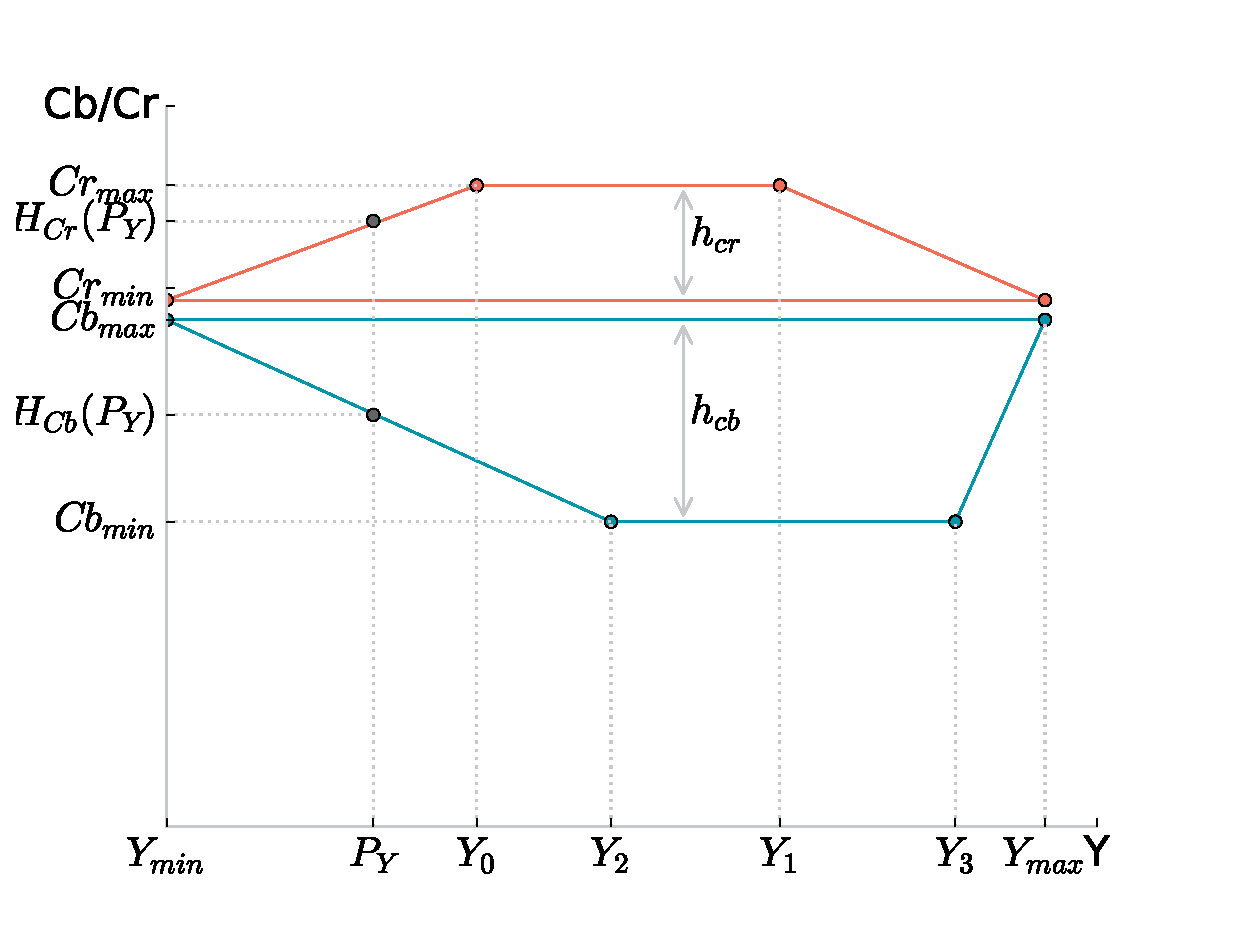
\includegraphics[width=0.8\textwidth]{trapezoids}
    \caption[Graphical representation of the trapezoids as well as its parameters]{Graphical representation of the trapezoids as well as the parameters $Y_{min} = 0$, $Y_{max} = 255$, $Y_{0}$, $Y_{1}$, $Y_{2}$, $Y_{3}$, $Cr_{min}$, $Cr_{max}$, $Cb_{min}$, $Cb_{max}$, $h_{Cr}$, $h_{Cb}$, $H_{Cr}(P_Y)$, $H_{Cb}(P_Y)$. Source: adapted from \citep{brancati:17}.}
    \label{fig:trapezoids}
\end{figure}

The base of the trapezoids $T_{YCr}$ and $T_{YCb}$ (Fig.~\ref{fig:trapezoids}) are given by $(Y_{min}, Cr_{min})$ and $(Y_{min}, Cb_{max})$ in the $YCr$ and $YCb$ subspaces, respectively. The values $Cr_{min}$ = 133, $Cb_{max}$ = 128 were selected according to~\citet{chai:99} where a skin color map was designed using a histogram approach based on a given set of training images. Chai and Ngan observed that the Cr and Cb distributions of skin color falls in the ranges [133, 173] and [77, 127], respectively, regardless the skin color variation in different races. 

The $Cr_{max}$ parameter is calculated dynamically, taking into account the histogram of the pixels with $Cr$ values in the range $[Cr_{min}, 183]$, looking for the maximum value of $Cr$ associated with at least 0.1\%\footnote{In \citet{brancati:17} this rate is reported to be equal to 10\%. However, in the distributed source code we found the value 0.1\%, that we are using in the experiments.} of pixels in the image. The same applies to $Cb_{min}$, taking the histogram with $Cb$ values in the range $[77, Cb_{max}]$. $Y_0$ and $Y_1$ (shorter base of the upper trapezoid) are, respectively, the 5${th}$ and 95$th$ percentile of the luminance values associated with the pixels of the image with $Cr = Cr_{max}$. A similar procedure is used to find the values of the shorter base of the other trapezoid, $Y_2$ and $Y_3$ (see Fig.~\ref{fig:crmax_computation} for an example).

\begin{figure}[ht]
    \centering
    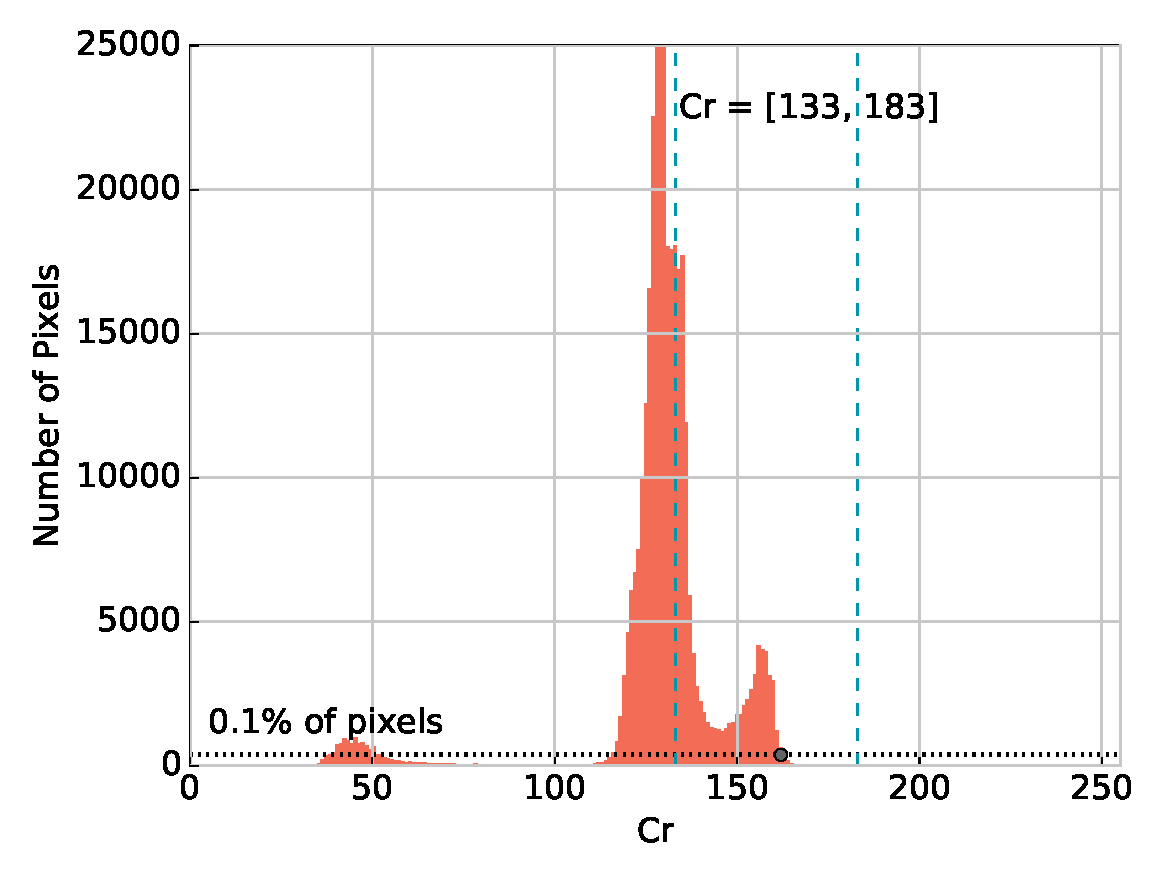
\includegraphics[width=0.7\textwidth]{crmax_computation}
    \caption[Computation of $Cr_{max}$ based on $Cr$ values histogram of a 724 x 526 image]{Computation of $Cr_{max} = 162$ based on $Cr$ values histogram of a 724 x 526 image.}
    \label{fig:crmax_computation}
\end{figure}

The correlation rules between the chrominance components $P_{Cr}$ and $P_{Cb}$ of a pixel $P$ are defined as:
\begin{itemize}
    \item the minimum difference between the values $P_{Cr}$ and $P_{Cb}$, denoted $I_P$;
    \item an estimated value of $P_{Cb}$, namely $P_{Cb_s}$;
    \item the maximum distance between the points $(P_Y, P_{Cb})$ and $(P_Y, P_{Cb_s})$, denoted $J_P$.
\end{itemize}

Therefore, to determine if $P$ is skin, the following equations must hold:
\begin{equation}
    P_{Cr} - P_{Cb} \geq I_P
\label{condition_c0}
\end{equation}
\begin{equation}
   |P_{Cb} - P_{Cb_s}| \leq J_P
\label{condition_c1}
\end{equation}

The estimated value $P_{Cb_{s}}$ is given by \footnote{$dP_{Cb_{s}}$ is the distance between the points $(P_Y, P_{Cb_{s}})$ and $(P_Y, Cb_{max})$ in the $YCb$ subspace, calculated on the basis of $dP_{Cr}$, observing the inversely proportional behavior of the components. $\alpha$ is the rate between the normalized heights of the trapezoids in relation to the $P_Y$ value.}:
\begin{equation}
    P_{Cb_s} = Cb_{max} - dP_{Cb_s}
\end{equation}
where \footnote{$dP_{Cr}$ is the distance between $(P_Y, P_{Cr})$ and $(P_Y, Cr_{min})$ points in the $YCr$ subspace.}:
\begin{align}
    dP_{Cb_s} &= \alpha \cdot dP_{Cr}
    \\
    dP_{Cr} &= P_{Cr} - Cr_{min}
\end{align}

The coordinates of the other sides of the trapezoids are given by $[P_Y, H_{Cr}(P_Y)]$ and $[P_Y, H_{Cb}(P_Y)]$, such that:
\begin{align}
  H_{Cr}(Y) &=  \begin{cases}
                Cr_{min} + h_{Cr}\big(\frac{Y - Y_{min}}{Y_0 - Y_{min}}\big) & Y \in [Y_{min},\ Y_0] \\
                Cr_{max} & Y \in [Y_0,\ Y_1] \\
                Cr_{min} + h_{Cr}\big(\frac{Y - Y_{max}}{Y_1 - Y_{max}}\big) & Y \in [Y_1,\ Y_{max}]
              \end{cases}
\\
  H_{Cb}(Y) &=  \begin{cases}
                Cb_{min} + h_{Cb}\big(\frac{Y - Y_2}{Y_{min} - Y_2}\big) & Y \in [Y_{min},\ Y_2] \\
                Cb_{min} & Y \in [Y_2,\ Y_3] \\
                Cb_{min} + h_{Cb}\big(\frac{Y - Y_3}{Y_{max} - Y_3}\big) & Y \in [Y_3,\ Y_{max}]
              \end{cases}
\end{align}

\noindent where $h_{Cr} = Cr_{max} - Cr_{min}$ and $h_{Cb} = Cb_{max} - Cb_{min}$, which are the heights of $T_{YCr}$ and $T_{YCb}$, respectively.

The computation of those points are useful for the calculation of $\alpha$. We first compute the distances $\Delta_{Cr}(P_Y)$ and $\Delta_{Cb}(P_Y)$ between the points $(P_Y, H_{Cr}(P_Y))$, $(P_Y, H_{Cb}(P_Y))$ and the base of the trapezoids:
\begin{align}
    \Delta_{Cr}(P_Y) &= H_{Cr}(P_Y) - Cr_{min} \\
    \Delta_{Cb}(P_Y) &= Cb_{max} - H_{Cb}(P_Y)
\end{align}

Next, the distances are normalized with respect to the difference in size of the trapezoids:
\begin{align}
  \Delta^{'}_{Cr}(P_Y) &=  \begin{cases}
                \Delta_{Cr}(P_Y) \cdot \frac{A_{T_{YCb}}} {A_{T_{YCr}}} &\quad \text{if}\ A_{T_{YCr}} \geq A_{T_{YCb}} \\
                \Delta_{Cr}(P_Y) &\quad \text{otherwise}
              \end{cases}
\\
  \Delta^{'}_{Cb}(P_Y) &=  \begin{cases}
                \Delta_{Cb}(P_Y) &\quad \text{if}\ A_{T_{YCr}} \geq A_{T_{YCb}} \\
                \Delta_{Cb}(P_Y) \cdot \frac{A_{T_{YCr}}} {A_{T_{YCb}}} &\quad \text{otherwise}
              \end{cases}
\end{align}
where $A_{T_{YCr}}$ and $A_{T_{YCb}}$ are the areas of trapezoid ${T_{YCr}}$ and ${T_{YCb}}$, respectively.

Then, the value of $\alpha$ is given by:
\begin{equation}
    \alpha = \frac{\Delta^{'}_{Cb}(P_Y)} {\Delta^{'}_{Cr}(P_Y)}
\end{equation}

Finally, $I_P$ and $J_P$ are given by:
\begin{equation}
    I_P = sf \cdot [(\Delta^{'}_{Cr}(P_Y) - dP_{Cr}) + (\Delta^{'}_{Cb}(P_Y) - dP_{Cb_s})]
    \label{eq:ip}
\end{equation}
\begin{equation}
    J_P = dP_{Cb_s} \cdot \frac{dP_{Cb_s} + dP_{Cr}} {\Delta^{'}_{Cb}(P_Y) + \Delta^{'}_{Cr}(P_Y)}
    \label{eq:jp}
\end{equation}
where:
\begin{equation}
    sf = \frac{min( (Y_1 - Y_0), (Y_3 - Y_2) )} {max( (Y_1 - Y_0), (Y_3 - Y_2) )}
\end{equation}

%% ------------------------------------------------------------------------- %%

\section{Extended Method}
\label{sec:proposed_method}
The hypothesis defined in the original method is based on rules that an estimated value of the point $P_{Cb}$, namely $P_{Cb_s}$, must hold in order for the correlation to be valid. On the basis of the inversely proportional behavior of the chrominance components, we will rewrite the correlation rules with respect to the $P_{Cr}$ point.

Thus, we have to refactor the correlation rules to put them in terms of the estimated value of $P_{Cr}$, that we denote as $P_{Cr_s}$ \footnote{$dP_{Cr_s}$ is the distance between the points $(P_Y, P_{Cr_s})$ and $(P_Y, Cr_{min})$ in the $YCr$ subspace, calculated on the basis of $dP_{Cb}$, observing the inversely proportional behavior of the components. $\alpha$ is the rate between the normalized heights of the trapezoids in relation to the $P_Y$ value.}:
\begin{equation}
    P_{Cr_s} = dP_{Cr_s} + Cr_{min}
\end{equation}
where \footnote{$dP_{Cb}$ is the distance between $(P_Y, P_{Cb})$ and $(P_Y, Cb_{max})$ points in the $YCb$ subspace.}:
\begin{equation}
    dP_{Cr_s} = \alpha \cdot dP_{Cb}
\end{equation}
\begin{equation}
    dP_{Cb}   = Cb_{max} - P_{Cb}
\end{equation}

Next, the constraints given by $I_P$ and $J_P$ in the Eq. \ref{eq:ip} and \ref{eq:jp} respectively, can be redefined as:
\begin{equation}
    I^{'}_P = sf \cdot [(\Delta^{'}_{Cr}(P_Y) - dP_{Cr_s}) + (\Delta^{'}_{Cb}(P_Y) - dP_{Cb})]
\end{equation}
\begin{equation}
    J^{'}_P = dP_{Cr_s} \cdot \frac{dP_{Cb} + dP_{Cr_s}} {\Delta^{'}_{Cb}(P_Y) + \Delta^{'}_{Cr}(P_Y)}
\end{equation}

Therefore, to determine if the pixel $P$ is skin, we have to modify the conditions given by Eq. \ref{condition_c0} and \ref{condition_c1}:
\begin{equation}
    P_{Cr} - P_{Cb} \geq I^{'}_P
\label{condition_c00}
\end{equation}
\begin{equation}
   |P_{Cr} - P_{Cr_s}| \leq J^{'}_P
\label{condition_c11}
\end{equation}

Doing this simple extension, we are now able to apply the method to the same sets of images to evaluate, in fact, the inversely proportional behavior of the chrominance components. More than that, we can combine all these constraints, given by the pair equations \ref{condition_c0} and \ref{condition_c1}, \ref{condition_c00} and \ref{condition_c11}, to reinforce the firstly defined hypothesis.


\begin{figure}[H]
    \centering
    \includegraphics[width=0.25\textwidth]{pixel_neighborhood}
    \caption[Neighbors evaluation with respect to a pixel $P$]{Neighbors evaluation with respect to $P$. If the image is scanned in raster order, $N_8^-(P)$ is the set of points that can be reached before $P$ in a 8-connected neighborhood.}
    \label{fig:pixel_neighborhood}
\end{figure}

%% ------------------------------------------------------------------------- %%

\section{Neighborhood Extended Method}
\label{sec:neighborhood_extended_method}
\noindent Both methods presented in Sec. \ref{sec:original_method} and \ref{sec:proposed_method} can be applied to detect skin pixels, either separated or in a conjunction rule. However, skin pixels do not usually appear isolated and we can improve the method using neighbor pixels information, when evaluating a pixel $P$, in order to decide if $P$ represents human skin, or not. Let $N_8^-(P)$ the 8-connected neighbors of $P$ that can be reached before $P$ when scanning the image in raster order (blue points in Fig.~\ref{fig:pixel_neighborhood}).

Thus, we classify $P$ as skin in the following manner: if the constraints given by the pair of equations \ref{condition_c0} and \ref{condition_c1}, as well as \ref{condition_c00} and \ref{condition_c11} hold, then $P$ is classified as skin. When only one of conditions is satisfied, then we check the decision in $N_8^-(P)$. If three or more pixels are skin, then $P$ will also be classified as a skin pixel.

%% ------------------------------------------------------------------------- %%

\section{Trapezoids Parameters Tuning with a Grid Search Strategy}
\label{sec:trapezoids_params_tunning}
\noindent As we could see on previous sections, this model is based on the definition of trapezoids to fit the skin color pixels distribution from a given image. According to~\citet{brancati:17}, the coordinates of each trapezoid within the $YCr$ and $YCb$ sub-spaces are calculated based on the $Y$ luminance component values. $Y_0$ and $Y_1$ are those used to define the shorter base of the upper trapezoid, and $Y_2$ and $Y_3$ the points used to define the shorter base of the lower trapezoid.

$Y_0$ and $Y_1$ are, respectively, the 5${th}$ and 95$th$ percentile of the luminance values associated with the pixels of the image with $Cr = Cr_{max}$ (see Fig.~\ref{fig:crmax_computation} for an example). Similarly, $Y_2$ and $Y_3$ are, respectively, the 5${th}$ and 95$th$ percentile of the luminance values associated with the pixels of the image with $Cb = Cb_{min}$.

To the best of our knowledge, there is any justification to choose the 5${th}$ and 95$th$ percentile to be the right parameters to define the trapezoids coordinates. For this reason, we decided to shot different combination of these parameters to figure out which pair better works for the model fitting. In addition, we would like to answer the question: why 5${th}$ and 95$th$ percentile have been used?

Thus, we used a well-known technique called grid search to find the best range combination from a hyper-parameter space. By constructing the model in this manner, we can leverage the classification results by finding the optimized parameters' combination, if other different from the ones defined earlier by \citet{brancati:17}. Despite we do not exhaustively consider all parameter combinations, we used an efficient search strategy by sampling a given number of candidates. For each chosen parameters candidate, we dynamically used them in the combined method\footnote{In fact, we could apply this approach in any of the described methods, but once the trapezoids definition do not change among them, we think that employing it only in combined method is sufficient for the parameters optimization.} to test every single image of each dataset described in section~\ref{sec:datasets}. Lastly, we sort the results table using respectively, $F-measure$, $Precision$, and $Recall$ metrics, as detailed in section~\ref{sec:evaluation_measures}, and established a comparison to get optimized parameters. The algorithm $\proc{Trapezoids-Parameters-Grid-Search}(dataset)$ shows how the grid search have been performed.

\begin{codebox}
\kern-1.5em $\proc{Trapezoids-Parameters-Grid-Search}(dataset)$\\
\li $Ymin \gets 5$
\li $Results \gets []$
\li \While $Ymin \leq 95$
\li \Do
        $Ymax \gets Ymin$
\li     \While $Ymax \leq 95$
\li     \Do
            $\proc{Set-Combined-Method-Y-Parameters}(Ymin, Ymax)$ \label{alg:tpgs-set-cmb-y}
\li         $\proc{Segment-Dataset-Images}(dataset)$    \label{alg:tpgs-segment-dtset}
\li         $Precision, Recall, Fmeasure \gets \proc{Compute-Metrics}(dataset)$ \label{alg:tpgs-compt-metrcs}
\li         $\proc{Push}(Results, Ymin, Ymax, Precision, Recall, Fmeasure)$ \label{alg:tpgs-push-rslts}
\li\li      $Ymax \gets Ymax + 5$
        \End
\li      $Ymin \gets Ymin + 5$
    \End
\li
\li $\proc{Sort-By}(Results, Fmeasure, Precision, Recall)$
\li \Return $Results$
\end{codebox}

In short, $\proc{Trapezoids-Parameters-Grid-Search}(dataset)$ will trigger combinations of $Ymin$ and $Ymax$ in the range $[5, 95]$ with a step of 5. In line~\ref{alg:tpgs-set-cmb-y}, the parameters are changed in the combined method and applied further in~\ref{alg:tpgs-segment-dtset} to classify each image within the dataset. Next, the metrics are computed on every single image in line \ref{alg:tpgs-compt-metrcs} by comparing the output with the ground truth. The resulting metrics are pushed into $Results$ matrix in line \ref{alg:tpgs-push-rslts} and sorted according the criteria aforementioned in the end of the procedure.

Detailed output of this experiments and analysis can be seen in chapter~\ref{cap:experimentos}, specifically in section~\ref{sec:grid_search_experiments}, where an examination of the behavior of the most performing parameters is given as well as others which did not succeed.